\documentclass[11pt, a4paper, oneside]{book}

% {{{ Packages
        \usepackage[margin=1in]{geometry}                           % Margins
          \linespread{1.2}                                          % Increases line spacing
        \usepackage{graphicx}                                       % Image Support
          \graphicspath{ {./images/} }                              % Path to image directory
        \usepackage{color}                                          % Colors for stuff
        \usepackage{soul}                                           % Provides Highlight feature
        \usepackage{fancyhdr}                                       % Fancy Header and footer
        \usepackage{amsmath}                                        % Math support
        \usepackage{amssymb}                                        % Extended symbols for math
        \usepackage{todonotes}                                      % Todo notes
        % \usepackage{etoolbox}                                       % IDK what it does. I just coppied it from stackexchage
        %   \AtBeginEnvironment{align}{\setcounter{equation}{0}}      % resets align counter for each instance
        \usepackage{listings}                                       % Code-snippet support
          % \definecolor{dkgreen}{rgb}{0,0.6,0}                     % lst-configs
          % \definecolor{gray}{rgb}{0.5,0.5,0.5}
          % \definecolor{mauve}{rgb}{0.58,0,0.82}

          % \lstset{                                                % lst-format-config
          %   frame=tb,
          %   language=Java,
          %   aboveskip=3mm,
          %   belowskip=3mm,
          %   showstringspaces=false,
          %   columns=flexible,
          %   basicstyle={\small\ttfamily},
          %   numbers=none,
          %   numberstyle=\tiny\color{gray},
          %   keywordstyle=\color{blue},
          %   commentstyle=\color{dkgreen},
          %   stringstyle=\color{mauve},
          %   breaklines=true,
          %   breakatwhitespace=true,
          %   tabsize=3
          % }
        \usepackage{caption}                                      % Caption support
        \usepackage[utf8]{inputenc}                               % utf encoding
        \usepackage{hyperref}
          \hypersetup{pdfnewwindow=true, colorlinks=false}
% }}}

% {{{ Footer section
        % Creates footer
        \pagestyle{fancy}%
        \fancyhf{}%
        \lfoot{Swapnil}%
        \cfoot{iamb4uc.xyz}%
        \rfoot{Page \thepage}%
        \renewcommand{\headrulewidth}{0pt}% Line at the head invisible
        \renewcommand{\footrulewidth}{0.4pt}% Line at the footer visible

        % Redefine the plain page style for chapter pages
        \fancypagestyle{plain}{%
          \fancyhf{}%
          \fancyfoot[L]{Swapnil}%
          \fancyfoot[C]{iamb4uc.xyz}%
          \fancyfoot[R]{Page \thepage}%
          \renewcommand{\headrulewidth}{0pt}% Line at the head invisible
          \renewcommand{\footrulewidth}{0.4pt}% Line at the footer visible
        }
% }}}

% {{{ Title
        \title{\Huge{\emph{Numerical and Statistical Analysis}}}
        \author{\huge{by \emph{Swapnil}}\\ \\ \Large{written in {\LaTeX}}}
        \date{\today}
% }}}

\begin{document}
%{{{ Title page
      \maketitle
      \thispagestyle{empty}
      \newpage
% }}}

%{{{ ToC
      \setcounter{tocdepth}{3}
      \tableofcontents
% }}}



%%%%%%%%%%%%%%%%%%%%%%%%%%%%%%%%%%%%%%%%%%%%%%%%%%%%%%%%%%%%%%%%%%%%%%%%%%%%%%%%%%%%%%%%%%%
%%%%%%%%%%%%%%%%%%%%%%%%%%%%%%%%%%%%%% Document Body %%%%%%%%%%%%%%%%%%%%%%%%%%%%%%%%%%%%%%
%%%%%%%%%%%%%%%%%%%%%%%%%%%%%%%%%%%%%%%%%%%%%%%%%%%%%%%%%%%%%%%%%%%%%%%%%%%%%%%%%%%%%%%%%%%
  %{{{
      \chapter{}
        \section{Errors in Numerical calculations}
          An error, in numerical calculations, is the difference between a true value and
          an estimate, or approximation, of that value.

          There are three main sources of errors in numerical computation:

          \textbf{\underline{rounding}, \underline{data uncertainty}, and
          \underline{truncation.}}

          \subsection{Rounding error}
            Rounding errors, also called arithmetic errors, are an unavoidable consequence of
            working in finite precision arithmetic. We will deal with these errors in the context
            of polynomial evaluation and solving linear equations.

          \subsection{Data Uncertainty}
            Uncertainty in the data is always a possibility when we are solving practical problems.
            It may arise in several ways: from errors in measuring physical quantities, from errors
            in storing the data on the computer (rounding errors), or, if the data is itself the
            solution to another problem, it may be the result of errors in an earlier computation.

          \subsection{Truncation}
            \textbf{Truncation} or \textbf{Discretization} or \textbf{Approximation errors} are much
            harder to analyze. We will deal with them in the context of solving differential equations.
            Many standard numerical methods (for example, the trapezoidal rule for quadrature,
            Euler's method for differential equations, and Newton's method for nonlinear equations) can
            be derived by taking finitely many terms of a Taylor series.

          \subsection{Approximation error}
            In numerical and statistical analysis, many results are only approximate; meaning they are
            similar but not equal to the actual result. An approximation can turn a complex calculation
            into a less complicated one.


        \section{Different types of errors}
          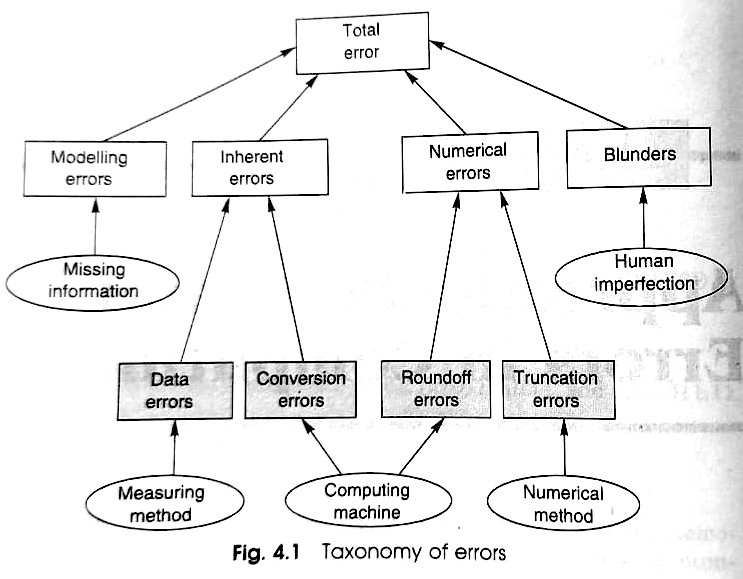
\includegraphics[scale=1.7]{toe.jpeg}

        \section{Significant Digit}
          The concept of significant digits has been introduced primarily to indicate the accuracy of a
          numerical value.

          If in the number y=23.40657, only the digits 23406 are correct,

          \noindent then we may say that y has five significant digits and is correct to only three decimal
          places.

          e.g. suppose we write 2/7 as 0.285714 and pie \( \) as 3.14159.

          \noindent Then we say the numbers contain six significant digits.


        \section{Accuracy}
          It is the closeness of the measured value to a standard or true value.

          In other way we say that accuracy is definedas `the degree to which the result of a measurement conforms
          to the correct value or a standard' and essentially refers to how close close a measurement is to its
          agreed value.

        \section{Precision}
          Precision is defined as ‘the quality of being exact’ and refers to how close two or more measurements
          are to each other, regardless of whether those measurements are accurate or not. It is possible for
          precision measurements to not be accurate.

        \subsection{Difference between Accuracy and Precision}
          Both accuracy and precision reflect how close a measurement is to an actual value, but they are not the
          same. Accuracy reflects how close a measurement is to a known or accepted value, while precision reflects
          how reproducible measurements are, even if they are far from the accepted value. Measurements that are
          both precise and accurate are repeatable and very close to true values.

          The concept of accuracy and precision are closely related to significant digits. They are related as follows:

          \begin{enumerate}
          \item Accuracy refers to the number of significant digits in a value. For example, the number 57.396 is
            accurate to fice significant digits \(sd\)

          \item Precision refers to the number of decimal positions, i\.e\. the order of magnitude of the
            last digit in a value. The number 57.396 has a precision of 0.001 or $10^{-3}$
          \end{enumerate}

        \section{Inherent errors}
          \textit{Inherent errors} are those that are present in the data supplied in \todo{Fill up the missing word}
          the model. Inherent errors (also known as input errors) contain two components, namely, data errors
          and conversion errors.

        % \section{Round-off error}


        \section{Different types of inherent errors encountered in numerical calcualtions}
        \begin{enumerate}
          \item \textbf{Data Error}: Data error (also known as \textit{empirical error}) arises when data for a
            problem are obtained by some experimental means and are, therefore, of limited accuracy and precision.
            This may be due to some limitations in instrumentation and reading, and therefore may be unavoidable.
            A physical measurement, such as a distance, a voltage, or a time period, cannot be exact. It is, therefore,
            important to remember that there is no use in performing arithmetic operations to, say, four decimal
            places when the original data themselves are only correct to two decimal places. For instance, the scale
            reading in a weighing machine may be accurate to only one decimal place.

          \item \textbf{Conversion Error}: Conversion errors(also known as \textit{representation errors})
            arises due to the limitations of the computer to store the data exactly. We know that the floating
            point representation retains only a specified number of digits. The digits that are not retained
            constitute the round-off error.

            As we have already seen, many numbers  cannot be represented exactly in a given number of decimal digits.
            In some cases a decimal number cannot be represented exactly in a binary form. For example, the decimal
            number 0.1 has a non-terminating binary form like 0.00011001100110011\dots but the computer retains only
            a specified number of bits. Thus, if we add 10 such numbers in a computer, the result will not be exactly
            1.0 because of round-off error during the conversion of 0.1 to binary from.

        \end{enumerate}


        \section{Chopping}
          In chopping, the extra digits are dropped this is called truncating the number.

          For example: \textit{A number like 42.7893 can be chopped as 42.78 i.e. the digits `93' will be dropped}

        \subsection*{Express the number 42.7893 in floating point form}

          % Equation
          \begin{align*}
          let,\ x &= 42.7893\\
          Now,\ x &= 0.427893 * 10^2\\
                  &= (0.4278 + 0.000093) * 10^2\\
                  &= (0.4278+0.93 * 10^{-4}) * 10^2\\
          This\ can\ be\ expressed\ in\ general\ form\\ as\ True\
                x &= (f_x + g_x + 10^{-d})10^E\\
                  &= f_x * 10^E + g_x * 10^{E-d}\\
                  &= approximate\ x + error\\
          \end{align*}

          where $f_x$ is the mantissa, d is the length of the mantissa permitted, E is the exponent in chopping $g_n$
          is ignored entirely and therefore error = $g_n * 10^{E-d}$ where $g_n \leq 1$


        \section{Error Analysis}
          \subsection{What do you mean by absolute and relative errors? Explain with examples.}
            Let us suppose that the true value of a data item is denoted by $x_t$ and its approximate value is denoted by
            $x_a$. Then, they are related as follows:

            \begin{equation*}
              True\ value\ x_t = Approximate\ value\ x_a + Error.
            \end{equation*}

            The error is then given by

            \begin{equation*}
              Error = x_t-x_a
            \end{equation*}

            The error may be negative or positive depending on the values of $x_t$ and $x_a$. In error analysis, what is
            important is the magnitude of the error \textit{absolute error} which is denoted by

            \begin{equation*}
              e = \left | x_t-x_a \right |
            \end{equation*}

            The relative error is defined as follows:

            \begin{align*}
              e_r &= \frac{absolute\ error}{\left | true\ value \right |}\\
                  &= \frac{\left | x_t-x_a \right |}{\left | x_t \right |} = \begin{vmatrix}
                                                                               1 -\frac{x_a}{x_t}
                                                                             \end{vmatrix}
            \end{align*}

            \subsubsection{Example 1.1}
              A civil engineer has measured the height of a 10 floor building as 2950 cm and the working height of each beam
              as 35 cm while the true values are 2945 cm and 30 cm respectively. Compare their absolute and relative errors

              Absolute error in measuring the height of the building is
              \begin{equation*}
                e_i=2950-2945=5\ cm
              \end{equation*}

              The relative error is

              \begin{equation*}
                e_{r,1}=\frac{5}{2945}=0.0017=0.17\%
              \end{equation*}

              Absolute error in measuring the height of the beam is

              \begin{equation*}
                e_2=35-30=5 cm
              \end{equation*}

              The relative error is

              \begin{equation*}
                e_{r,2}=\frac{5}{30}=0.17=17\%
              \end{equation*}


        \section{Percentage error}
          The fractional form of $e_r$ can also be expressed as the
          \textit{percent relative error} as

        \begin{equation*}
        Percent\ e_r=e_r*100
        \end{equation*}

          \subsection{Examples}
            \subsubsection{Example 1.2}
              Suppose that the in measurement of inner diameter of the pipe reading
              obtained using vernier calliper is $l=2.00\pm0.05$ cm, then the relative
              error and percentage error is given as,

            \subsubsection{Example 1.3}
              An approximate value of $\pi$ is given by $X_1=\frac{22}{7}=3.1428571$
              and its true value is $X=3.1415926$. Find the absolute and relative errors.
              We have

              \begin{equation*}
                E_A=X-X_1=-0.0012645\ and\ E_R=\frac{-0.0012645}{3.1415926}=-0.000402
              \end{equation*}

            \subsubsection{Example 1.4}
              Three approximate values of the number $\frac{1}{3}$ are given as 0.30, 0.33
              and 0.34. Which of these three is the best approximation? We have

              \begin{align*}
                \begin{vmatrix}
                  \frac{1}{3}-0.30
                \end{vmatrix} &= \frac{1}{30},\\
              \\
                \begin{vmatrix}
                  \frac{1}{3}-0.33
                \end{vmatrix} &= \frac{0.01}{3},=\frac{1}{300},\\
              \\
                \begin{vmatrix}
                  \frac{1}{3}-0.34
                \end{vmatrix} &= \frac{0.02}{3}=\frac{1}{150}
              \end{align*}

              It follows that 0.33 is the best approximation for $\frac{1}{3}$

            \subsubsection{Example 1.5}
              Find the relative error of the number 8.6 if both of its digits are correct.
              Here

              \begin{align*}
                        E_A &= 0.05 \\
                Hence,\ E_R &= \frac{0.05}{8.6}=0.0058
              \end{align*}

            \subsubsection{Example 1.6}
              Evaluate the sum $S = \sqrt{3} + \sqrt{5} + \sqrt{7}$ to 4 significant digits and
              find it's absolute and relative errors. We have

              \begin{equation*}
              \sqrt{3}=1.732,\ \sqrt{5}=2.236,\ \sqrt{7}=2.646
              \end{equation*}

              Hence $S=6.614$

              \begin{align*}
                and\ E_A &= 0.0005+0.0005+0.0005 \\
                         &= 0.0015
              \end{align*}

              The total absolute error shows that the sum is correct to 3 significant figures only.
              Hence, we take $S=6.61$ and then $E_R=\frac{0.0015}{6.61}=0.0002$

          \subsection{Difference between absolute, relative and percentage error}
            \Large{\texttt{Absolute error = |True Value - Measured Value|}}

            Absolute error is the magnitude of the difference between a measurement
            compared to a true value.

            \noindent \Large{\texttt{Relative Error = Absolute Error/True Value}}

            Relative error shows the size of error relative to the true value. Basically,
            it puts the size of the error into perspective.

            \noindent \Large{\texttt{Percent Error=Relative Error * 100\%}}

            Percent error shows what percent the error is of the true or accepted value.


        \section{Transcendental Equation}
          By the help of algebraic approach we can solve equations of all degrees upto and
          including the $4^{th}$ degree and it is also known how to compute the rules of
          numerical equations of any degree. Algebra is silent however, on the solution of
          such type of equation as $ax+b\log{x}+c=0$ or $ae^x+b\tan{x}=c$ etc. These are
          called transcendental equations and no general method exists for finding their
          roots in terms of their coefficient. When the coefficient of such equations are
          pure numbers, it is always possible to compute the roots to any degree of accuracy.

          \subsection{Bisection method}
            This method of solving a transcendental equation consists in locating the roots
            of the equation $f(x)=0$ between two numbers, say $x_0$ and $x_1$, such that
            $f(x)$ is continuous for $x_0\leq x\leq x_1$ and $f(x_0)$ and $f(x_1)$ are the
            opposite signs so that $f(x_0)*f(x_1)<0$ i.e., the curve crosses the x-axis between
            $x_0$ and $x_1$ and the desire roof of the given equation is approximately,

            \begin{align*}
              x_2&=\frac{x_0+x_1}{2}\\
              x_3&=\frac{x_0+x_2}{2},\ provided\ f(x_0)*f(x_2)<0\\
              &=\frac{x_1+x_2}{2},\ provided\ f(x_1)*f(x_2)<0\\
              Further\ x_4&=\frac{x_0+x_3}{2},\ provided\ f(x_0)*f(x_3)<0
            \end{align*}

            and so on

            Thus, on each iteration, we find the root with desired accuracy or we narrow down
            the range to half of the previous interval.


          \subsection{Newton + Raphson method}
            When the derivative of f(x) is a simple expression and easily found, the real root
            of $f(x)=0$ can be computed rapidly by a process called the Newton-Raphson method.
            The underlying idea of the method is due to Newton, but the method as now used is
            due to Raphson.

            To derive a formula for computing real roots by this method, let \textit{a} denote
            an approximate value of the desire root and also let \textit{h} is the correlation
            which is applied to \textit{a} to get the exact value of the root of the given
            equation so that $x=a+h$

            The equation $f(x)=0$, then

            \begin{equation*}
              f(a+h)=0
            \end{equation*}

            Expanding by Taylor's theorem, we get,
            \begin{align*}
                                                           f(a+h) &= f(a)+hf'(a)+
                                                                     \frac{h^2}{2}f''(a+\theta h),\
                                                                     0\le \theta \le 1\\
                                                                  &= 0\\
              \therefore f(a)+hf'(a)+\frac{h^2}{2}f''(a+\theta h) &= 0
            \end{align*}

            Now if h is very small, we can neglect the term containing $h^2$ and as such

            \begin{align*}
                                    f(a)+hf'(a) &= 0\\
              \Rightarrow h=\frac{-f(a)}{f'(a)} &= h_1(say)\rightarrow (I)
            \end{align*}

            The improved value of the root is then

            \begin{equation*}
              a_1=a+h_1=a-\frac{f(a)}{f'(a)}
            \end{equation*}

            The succeeding approximation are
            \begin{align*}
                          a_2=a_1+h_2 &= a_1-\frac{f(a_1)}{f'(a_1)}\\
              Similarly,\ a_3=a_2+h_3 &= a_2-\frac{f(a_2)}{f'(a_2)}\\
                      a_n=a_{n-1}+h_n &= a_{n-1}-\frac{f(a_{n-1})}{f'(a_{n-1})}
            \end{align*}

            Equation \textit{(I)} is the fundamental formula in the Newton-Raphson method.
            It is evident from this formula that larger the derivative $f'(x)$, the smaller
            the correlation which must be applied to get the correct root of the equation.
            This means that when the graph is nearly vertical, where it crosses the x-axis,
            the correct the value of the root can be found with great rapidity and very little
            labour. On the other hand, when the graph is horizontal on the x-axis, the Newton-Raphson
            method will be a slow process for computing the real root of the given equation
            or might even fail.

            The Newton-Raphson method should never be used when the graph of $f(x)$ is nearly
            horizontal where it crosses the x-axis.

          \subsection{Method of false position/Regular falsi method}
            The oldest method for computing the real roots of a numerical equation is the method
            of false position. In this method, we find two numbers $x_1$ and $x_2$ between which
            the root lies. This numbers should be as close as possible. Since the root lies
            between $x=x_1$ and $x=x_2$ and $f(x_1)$ and $f(x_2)$ must have opposite sign.

            Now, since any position of a smooth curve is practical straight for a short distant,
            it is legitimate to assume that the change in $f(x)$ is proportional to the change in
            x over a short interval. The method of false position is based on this principle because
            it assumes that the graph of $y=f(x)$ is straight line between the point $(x_1,y_1)$ and
            $(x_2,y_2)$, these points are on the opposite side of the x-axis.

            To derive a formula for computing the root of the given equation let the following
            figure represent a magnified view of that part of the graph \{between $(x_1,y_1)+(x_2,y_2)$\}
            where it chooses the x-axis, i.e., between which the root lies.

            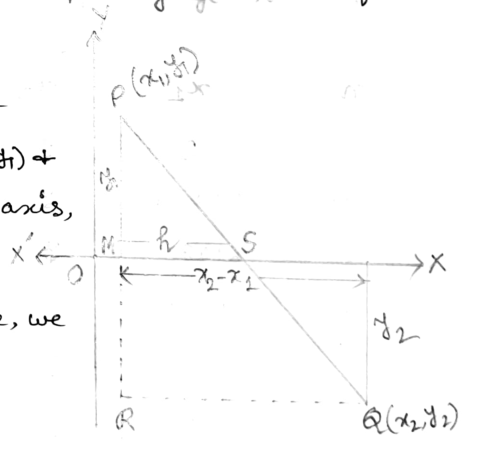
\includegraphics{mofdiagram}

            From the similar triangle, we have,

            \begin{align*}
                            \frac{MS}{RQ} &= \frac{PM}{PR}\\
              \Rightarrow   \frac{MS}{PM} &= \frac{RQ}{PR}\\
              \Rightarrow \frac{h}{|y_1|} &= \frac{x_2-x_1}{|y_1|+|y_2|}\\
              \Rightarrow               h &= \frac{(x_2-x_1)*|y_1|}{|y_1|+|y_2|}
                                           = \frac{(x_2-x_1)*|f(x_1)|}{|f(x_1)|+|f(x_2)|}
                                             \ \ \ \ \ [\because y=f(x)]
            \end{align*}

            The value of the desire root under the assumption made
            \begin{align*}
              x &= x_1+h\\
                &= x_1+\frac{(x_2-x_1)*|f(x_1)|}{|f(x_1)|+|f(x_2)|}
            \end{align*}

            This value of x however not the true value of the root because the graph of $y-f(x)$
            is not perfectly a straight line between $(x_1,y_1)$ and $(x_2,y_2)$. It is nearly a
            closer approximation to the true root.

          \section*{Questions}%{{{
              % \item \large \textbf{\textit{Discuss absolute error, relative error and percentage error with an example for each.}}\normalsize{{{{{{
              % \item \large \textbf{\textit{Given that
              %   \begin{align*}
              %     a&=10.00\pm0.05\\
              %     b&=0.0356\pm0.0002\\
              %     c&=15300\pm100\\
              %     d&=62000\pm500
              %   \end{align*}
              %   Find the maximum value of the absolute error in (\textit{i})$a+b+c$ and (\textit{ii})$c^3$.}}\normalsize

              % \subsection{What do you mean by normalized floating-point number? Give an example.}

              % \subsection{Perform the following floating-point operations:}
              %   \begin{enumerate}
              %     \item Add 0.863451 E2 and 0.653427 E5
              %     \item Add 0.964571 E3 and 0.725439 E-1
              %     \item Subtract 0.635742 E3 from 0.994576 E4
              %     \item Multiply 0.437263 E4 and 0.111000 E-2
              %     \item Divide 0.876543 E-5 by 0.200000 E-3
              %   \end{enumerate}
              % \item \large \textbf{\textit{Define significant digits, precision and accuracy, round-off error, approximation error.}}\normalsize
              % \item \large \textbf{\textit{Find the relative error and percentage error of the following numbers:}}\normalsize
              %   $$
              %   48.21416,\ 2.3742,\ 52.275
              %   $$

              % \item \large \textbf{\textit{Explain in brief the types of errors one might encounter in performing numerical calculations.}}\normalsize
              % \item \large \textbf{\textit{If $X=2.536$, find the absolute error and relative error when:}}\normalsize
              %   \begin{itemize}
              %     \item X is rounded;
              %     \item X is truncated to two decimal digits.
              %   \end{itemize}
              % \item \large \textbf{\textit{What is normalization in floating point arithmetic? Describe, with example, underflow and overflow.}}\normalsize
              % \item \large \textbf{\textit{Differentiate between relative error and absolute error. Which error is of the accumulative type and why?}}\normalsize}}}}}}
              \subsection{What do you mean by floating point representation? How we normalize the floating point value while doing addition and subtraction operations?}
                \textbf{Answer}

                Floating Point Arithmetic Operation:

                The floating point representation of a number has two parts. The first part represents a signed fixed point number called the \underline{mantissa}. The $2^{nd}$ part designates the position of the decimal point and is called the \underline{exponent}. The fixed point mantissa may be fraction or an
                integer.

                \textit{For example}:

                The decimal number `$+6132.789$' is represented in floating point with a fraction and an exponent as follows:\\

                \begin{tabular}{c c}
                  \underline{Fraction} & \underline{Exponent}\\
                   & \\
                  $+0.6132789$ & $+04$\\
                \end{tabular}

                The value of the exponent indicates the actual position of the decimal point is 4 positions to the right of the indicated decimal point in the fraction. Thus representation is equivalent to the scientific notation $+0.6132789 * 10^4$

                * Floating point is always interpreted to represent a number in the following form.
                $$
                m * r^e
                $$
                where m is the mantissa, r is the radix and e is the exponent.

                \textit{For example}: The binary number $+1001.11$ is represented with an 8-bit fraction and 6-bin expression as follows:\\

                \begin{tabular}{c c}
                  \underline{Fraction} & \underline{Exponent}\\
                   & \\
                  $01001110$ & $000100$\\
                \end{tabular}

                The fraction has zero in the left most position to denote \todo{Find the proper word for this space}. The exponent has the equivalent binary number +4. The floating point number is equivalent to $m*2^e=(0.1001110)*2^{+4}$

                $Arithmetic\ Operation\ \rightarrow (with\ floating\ point\ number)$
                \\ \\ \\
                \Large \textbf{Addition and Subtraction}\normalsize

                Assume a fractional representation and a radix 10. The decimal number 537.25 is represented in a register with $m=537.25$ and $e=3$ and is interpreted to represent the floating point number $0.53725*10^3$

                A floating point is \underline{normalized} if the most significant digit of the mantissa is non-zero.

                Arithmetic operations with floating point numbers are more complicated then with fixed point numbers and their execution takes longer and requires more complex hardware.

                \textit{For example}: Consider the sum of the following floating point numbers:

                \begin{equation*}
                0.5372400*10^2
                \end{equation*}
                \begin{equation*}
                0.1530000*10^{-1}
                \end{equation*}

                It is necessary that the two exponents equal before the mantissa can be added. That is why the about two number cannot be added
                \begin{equation*}
                  \left.\begin{matrix}
            0.5372400*10^2 \\ \underline{0.0001580*10^2} \\ 0.5373980*10^2
            \end{matrix}\right\}
                \end{equation*} \textbf{NOTE}: If there is any overflow then it should be shift the sum once to right and increase to exponent

                When two normalized mantissa are added the sum may contain a overflow digit. An overflow can be corrected easily by shifting the sum once to the right and incrementing the exponent.

                \textit{For example}: When two numbers are subtracted, the result may contain most significant zeros as shown in the following example:

                \begin{equation*}
                  \begin{matrix}
                    0.56780*10^5 \\
                    \underline{0.56430*10^5} \\
                    0.00350*10^5
                  \end{matrix}
                \end{equation*}
                \textbf{NOTE}: In this case we have to shift the mantissa and just decrease the exponent

                A floating point number that has a zero in the most significant position of the mantissa is said to have an underflow. To normalise a number that contains an underflow it is necessary to shift the mantissa to the left and decrement the exponent until a non-zero digit in the $1^{st}$ position.

                \textit{For example}: In the above floating point number it is necessary to shift left twice to obtain the
                \begin{equation*}
                  0.35000*10^3
                \end{equation*}


              \subsection{Find the root of the equation by Bisection method}
              \begin{enumerate}
              \item $x^3-2x-5=0$

              \textbf{Answer}

              Given,
              \begin{align*}
              f(x)&=x^3-2x-5\\
              \therefore f(1)&=-6\\
              f(2)&=-1\\
              f(3)&=16
              \end{align*}
              $\therefore$ Root of the given equation lies between 2 and 3

              \Large
             \begin{center}
            \begin{tabular}{|l|l|l|l|l|}
            \hline
              n  & a     & b     & $x=\frac{a+b}{2}$ & $f(x)$ ie, $f\frac{a+b}{2}$ \\ \hline
              1  & 2     & 3     & 2.5               & 5.625                       \\ \hline
              2  & 2     & 2.5   & 2.25              & 1.891                       \\ \hline
              3  & 2     & 2.25  & 2.125             & 0.346                       \\ \hline
              4  & 2     & 2.125 & 2.063             & -0.346                      \\ \hline
              5  & 2.063 & 2.125 & 2.094             & -0.006                      \\ \hline
              6  & 2.094 & 2.125 & 2.110             & 0.174                       \\ \hline
              7  & 2.094 & 2.110 & 2.102             & 0.083                       \\ \hline
              8  & 2.094 & 2.102 & 2.098             & 0.039                       \\ \hline
              9  & 2.094 & 2.098 & 2.096             & 0.016                       \\ \hline
              10 & 2.094 & 2.096 & 2.095             & 0.005                       \\ \hline
              11 & 2.094 & 2.095 & 2.095             & 0.005                       \\ \hline
            \end{tabular}
            \end{center}
            \normalsize

            Since, in the $10^{th}$ and $11^{th}$ iteration, the value of x is the same.

            $\therefore$ The root of the given equation is approximately 2.095

            \item $x^3-x-1=0$

              \textbf{Answer}

                  Given,
                  \begin{align*}
                    f(x)&=x^3-x-1\\
                    \therefore f(1)&=-1\\
                    f(2)&=5\\
                  \end{align*}
                  $\therefore$ Root of the given equation lies between 1 and 2
                  \Large
                  \begin{center}
                  \begin{tabular}{|l|l|l|l|l|}
                    \hline
                    n  & a     & b     & $x=\frac{a+b}{2}$ & $f(x)$ ie, $f\frac{a+b}{2}$ \\ \hline
                    1  & 1     & 2     & 1.5               & 0.875                       \\ \hline
                    2  & 1     & 1.5   & 1.25              & -0.295                      \\ \hline
                    3  & 1.25  & 1.3   & 1.375             & 0.225                       \\ \hline
                    4  & 1.25  & 1.375 & 1.313             & -0.049                      \\ \hline
                    5  & 1.313 & 1.375 & 1.344             & 0.084                       \\ \hline
                    6  & 1.313 & 1.344 & 1.329             & 0.018                       \\ \hline
                    7  & 1.313 & 1.329 & 1.321             & -0.016                      \\ \hline
                    8  & 1.321 & 1.329 & 1.325             & 0.001                       \\ \hline
                    9  & 1.321 & 1.325 & 1.323             & -0.007                      \\ \hline
                    10 & 1.323 & 1.325 & 1.324             & -0.003                      \\ \hline
                    11 & 1.324 & 1.325 & 1.325             & 0.001                       \\ \hline
                    12 & 1.324 & 1.325 & 1.325             & 0.001                       \\ \hline
                  \end{tabular}
                  \end{center}
                  \normalsize

                  Since, in the $11^{th}$ and $12^{th}$ iteration, the value of x is same.

                  $\therefore$ The root of the given equation is 1.325
            \end{enumerate}

            \subsection{By using Newton-Raphson method, find the root of }
              \begin{enumerate}
                \item $x^4-x-10=0$

                  \textbf{Solution}

                  Given,
                  \begin{align*}
                    f(x)&=x^4-x-10\\
                    \therefore f'(x)&=4x^3-1\\
                    Let,\ x_0&=2\\
                    \therefore f(x_0)=4\ and&\ f'(x_0)=31
                  \end{align*}
                  Now,
                  \begin{align*}
                    x_1&=x_0-\frac{f(x_0)}{f'(x_0)}\\
                    &=2-\frac{4}{31}\\
                    &=1.871\\
                    f(x_1)&=0.383\ and\ f'(x_1)=25.199\\
                    \therefore x_2&=x_1-\frac{f(x_1)}{f'(x_1)}\\
                    &=1.871-\frac{0.383}{25.199}\\
                    &=1.856\\
                    f(x_2)&=0.010\ and\ f'(x_2)=24.574\\
                    \therefore x_3&=x_2-\frac{f(x_2)}{f'(x_2)}\\
                    &=1.856-\frac{0.010}{24.574}\\
                    &=1.856\\
                  \end{align*}
                  $\because$ In the $2^{nd}$ and $3^{rd}$ iteration, the value of x is sam

                  $\therefore$ Root of the given equation is 1.856\\
                  \ \\
                \item $x^6=x^4+x^3+1$

                  \textbf{Solution}

                  \begin{align*}
                    x^6&=x^4+x^3+1\\
                    \Rightarrow &x^6-x^4-x^3-1=0\\
                    \therefore f(x)&=x^6-x^4-x^3-1\\
                    f'(x)&=6x^5-4x^3-3x^2\\
                  \end{align*}

                    Let $x_0=2$

                  \begin{align*}
                    \therefore f(x_0)&=39\ and\ f'(x_0)=148\\
                    \therefore x_1&=x_0-\frac{f(x_0)}{f'(x_0)}\\
                    &=2-\frac{39}{148}
                  \end{align*}

                  \hl{To be continued}
              \end{enumerate}



            %}}}

  % }}}
  %{{{
      \chapter{}
       \section{Calculas of finite difference}
         The calculas of finite difference deals with the changes in the values of the
         dependent variable due to the changes in the independent variable.

         Let, `$y$' be a function of `x' represented by $y=f(x)$. Let, $a,a+h,a+2h,
         \dots,(a+nh)$ be the $(n+1)$ equidistant values of x and
         $f(a),f(a+h),f(a+2h),\dots,f(a+nh)$ be the corresponding values of $f(x)$.

         The values of $x$ are called arguments and the values of $f(x)$ are called
         entries.

         Again,

         \begin{align*}
           (a+h)-a&=(a+2h)-(a+h)=(a+3h)-(a+2h)=\dots\\
           &=(a+nh)-\{a+(n-1)h\}\\
           &=h
         \end{align*}

         where, `h' is called the interval of differences.

         \begin{enumerate}
           \item Difference of first order($\Delta$)

             \begin{equation*}
               \Delta f(x)=f(x+h)-f(x)
             \end{equation*}

           \item Difference of second order($\Delta^2$)

             \begin{align*}
               \Delta^2 f(x)&=\Delta \{\Delta f(x)\}\\
               &=\Delta \{f(x+h)-f(x)\}\\
               &=\Delta f(x+h)-\Delta f(x)\\
               &=f(x+2h)-f(x+h)-\{f(x+h)-f(x)\}\\
               \Delta^2f(x)&=f(x+2h)-2f(x+h)+f(x)\\
             \end{align*}

           \item Difference of second order($\Delta^3$)

             \begin{align*}
               \Delta^3 f(x)&=\Delta \{\Delta^2 f(x)\}\\
               &=\Delta \{f(x+2h)-2f(x+h)+f(x)\}\\
               &=f(x+3h)-f(x+2h)-2f(x+2h)+2f(x+h)+f(x+h)-f(x)\\
               &=f(x+3h)-3f(x+2h)+3f(x+h)-f(x)
             \end{align*}

         \end{enumerate}


       \section{Difference Table}
         When we arrange the difference of various orders of a function systematically
         along with arguments and entries in a table, then its is known as diffrence table.

         Let, $x_0,x_1,x_2,x_3$ are 4 equidistant values of x such that $x_1-x_0,x_2-x_1,x_3-x_2=h$
         and $f(x_0),f(x_1),f(x_2),f(x_3)$ are the corresponding values of $f(x)$,
         then the difference table is

         % 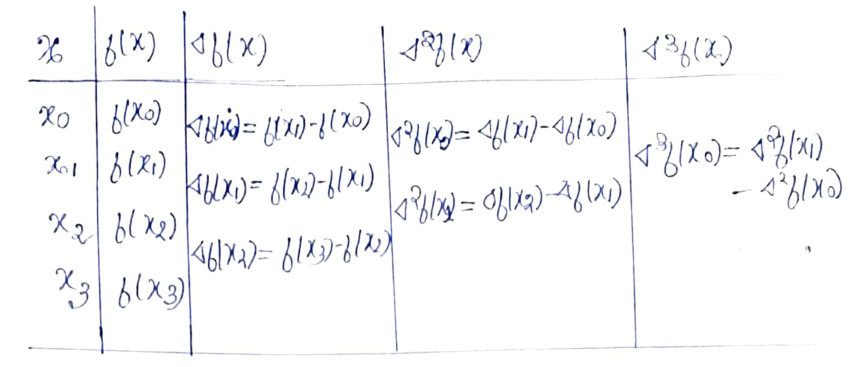
\includegraphics[scale=0.65]{difference table}


       \section{Interpolation}
         Interpolation is a technique of estimating the approximates of the value
         of the depending variable corresponding to a value of the independent variable,
         between its two extreme values, on the basis of the given independent and
         dependent variables values.

       \section{Assumption of interpolation}
         The application of principal of interpolation is subject to the following assumption.
         \begin{itemize}
           \item There is no sudden jumps in figures from one period to another period.

           \item The rate of change of figure is uniform, over-time.

         \end{itemize}
       \section{Different Interpolation formulae}
         \subsection{Newton's forward interpolation formula}
           It is used to estimate the value of the dependent variable corresponding to
           a given value of the independent variable, if:

           \begin{enumerate}
             \item The independent variable $x$, increases by equal intervals.
             \item The value of $x$, correponing which the value of $y$ us to be interpolated in the first hub of the series.
           \end{enumerate}

           The formula is

           \begin{align*}
             f(x)=f(x_0)+U\Delta f(x_0)&+\frac{U(U-1)}{2!}\Delta^2f(x_0)+\frac{U(U-1)(U-2)}{3!}\Delta^3f(x_0)\\
             &+\dots+\frac{U(U-1)(U-2)\dots\{U-(n-1)\}}{n!}\Delta^nf(x_0)\\
           \end{align*}

           where $U=(\frac{x-x_0}{h})$ and h is the interval of differencing.

           \subsubsection{Derivation}{{{
           Let, $y=f(x)$, be a function,

           Here, the argument's $x_0,x_1,\dots.x_n$ are equidistant. $x_1-x_0=x_2-x_1=\dots=x_n-x_{n-1}=h$

           Let us take a polynomial of $n^{th}$ degree as our interpolation formula.

           Let
           \begin{equation}\label{dv1}
             f(x)=a_0+a_1(x-x_0)+a_2(x-x_0)(x-x_1)+\dots+a_3(x-x_0)(x-x_1)\dots(x-x_{n-1})
           \end{equation}
           where $a_0,a_1,\dots,a_n$ are the constants to be determined.

           Now, putting $x=x_0$ in equation number (\ref{dv1})
           \begin{align*}
             f(x_0)&=a_0
           \end{align*}
           Again, putting $x=x_1$ in equation (\ref{dv1})
           \begin{align*}
             f(x_1)&=a_0+a_1(x_1-x_0)\\
             \Rightarrow f(x_1)&=f(x_0)+a_1*h\\
             \Rightarrow a_1 &=\frac{f(x_1)-f(x_0)}{h}\\
             &=\frac{\Delta f(x_0)}{h}
           \end{align*}

           Again, putting $x=x_2$ in equation (\ref{dv1})
           \begin{align*}
                         f(x_2)  &= a_0+a_1(x_2-x_0)+a_2(x_2-x_0)(x_2-x_1)\\
             \Rightarrow f(x_2)  &= f(x_0)+\frac{\Delta f(x_0)}{h}(x_2-x_1+x_1-x_0)\\ &+ a_2(x_2-x_1+x_1-x_0)(x_2-x_1)\\
             \Rightarrow f(x_2)  &= f(x_0)+\frac{\Delta f(x_0)}{h}*2h+a_2*2h*h\\
             \Rightarrow f(x_2)  &= f(x_0)+2\Delta f(x_0)+2h^2a_2\\
             \Rightarrow a_2     &= \frac{f(x_2)-2\Delta f(x_0)-f(x_0)}{2h^2}\\
             \Rightarrow a_2     &= \frac{f(x_2)-2f(x_1)+2f(x_0)-f(x_0)}{2h^2}\\
                                 &= \frac{f(x_2)-2f(x_1)+f(x_0)}{2!h^2}\\
                                 &= \frac{\Delta^2 f(x_0)}{2!h^2}
           \end{align*}

           Again, putting $x=x_3$ is equation (\ref{dv1})
           \begin{equation*}
             a_3=\frac{\Delta^3f(x_0)}{3!h^3}\\
           \end{equation*}

           ....................

           ....................................


           Similarly, putting $x=x_n$ in equation (\ref{dv1})
           \begin{equation*}
             a_n=\frac{\Delta^nf(x_0)}{n!h^n}
           \end{equation*}

           Now putting the value of $a_0,a_1,a_2,a_3,\dots,a_n$ in equation (\ref{dv1}), we get,
           \begin{equation*}\label{dv2}
             f(x)=f(x_0)+\frac{\Delta f(x_0)}{h}(x-x_0)+\frac{\Delta^2f(x_0)}{2!h^2}(x-x_0)(x-x_1)
           \end{equation*}
           \begin{equation*}\label{dv2}
                 +\frac{\Delta^3f(x_0)}{3!h^3}(x-x_0)(x-x_1)(x-x_2)
           \end{equation*}
           \begin{equation}\label{dv2}
                 +\dots+\frac{\Delta^nf(x_0)}{n!h^n}(x-x_0)(x-x_1)\dots(x-x_{n-1})
           \end{equation}

           Let us put $U=\frac{x-x_0}{h}$ in equation (\ref{dv2})
           \begin{align*}
             f(x)&=f(x_0)+U\Delta f(x_0)+\frac{U(U-1)}{2!}\Delta^2f(x_0)+\frac{U(U-1)(U-2)}{3!}\Delta^3f(x_0)\\
             &+\dots+\frac{U(U-1)\dots\{U-(n-1)\}}{n!}\Delta^nf(x_0)
           \end{align*}}}}

         \subsection{Newton's backward interpolation formula}
           Let, $f(x)$ be a polynomial  of degree $n$ and $n+1$ equidistant values of $x$ along then
           corresponding values of $f(x)$. The Newton's backward interpolation formula is

           \begin{align*}
             f(x) &= f(x_n)+U\nabla f(x_n-1)+\frac{U(U+1)}{2!}\nabla^2f(x_n-2)+\frac{U(U+1)(U+2)}{3!}\nabla^3f(x_n-3)\\
                  &+\dots+\frac{U(U+1)\dots\{U+(n-1)\}}{n!}\nabla^nf(x_0)
           \end{align*}

           where, $U=\frac{(x-x_n)}{h}$, where h is the interval of differences.

           The Newton's backward interpolation formula is used to estimate values of the dependent
           variable corresponding to a given value of the independent variable.

           \begin{enumerate}
             \item The independent variable $x$ increases by equal intervals.
             \item The value of $x$ corresponding to each value of $y$ is to be interpolated in
               the $2^{nd}$ half of the series.
           \end{enumerate}

         \subsection{Lagrenge's interpolation formula}
         Let, $f(x_0),f(x_1),\dots,f(x_n)$ be the entries corresponding to the argument
         $x_0,x_1,\dots,x_n$ which are not necessarily in equal intervals. The interpolation
         formula given by Lagrenge to estimate the value of $y$ corresponding to a value of $x$
         between any two consecutive values of the given values is

         \begin{align*}
           f(x)&=\frac{(x-x_1)(x-x_2)\dots(x-x_n)}{(x_0-x_1)(x_0-x_2)\dots(x_0-x_n)}f(x_0)+\frac{(x-x_0)(x-x_2)\dots(x-x_n)}{(x_1-x_0)(x_1-x_2)\dots(x_1-x_n)}f(x_1)\\
           &+ \dots +\frac{(x-x_1)(x-x_2)\dots(x-x_{n-1})}{(x_n-x_0)(x_n-x_1)\dots(x_n-x_{n-1})}f(x_n)
         \end{align*}

         Lagrange's Interpolation formula is usually and when the values of the independent
         variable $x$ are not equidistant. To apply Lagrange's formula the value of $x$
         corresponding to which the value of $y$ is to be interpolated may be anywhere in
         between the first and last terms.

         To apply Lagrange's formula, constuction of difference table is not needed.
  % }}}
  %{{{
      \chapter{}
        \section{Numerical Integration}
          Numerical Integration is the process of finding or evaluating definate integral is

          $I=\int_{a}^{b}f(x)dx$ from a set of numerical value of the integrant $f(x)$.
          If it is applied to the integration of a function of a single variable then the
          process is known as quadrature. The problem of numerical integration is solved by
          first approximating the integrant by a polynomial with the help of an interpolation
          formula and then integrating this expression between the desired limits.

          \begin{align*}
            \int xdx&=\frac{x^2}{2}\\
            \int x^ndx&=\frac{x^{n+1}}{n+1}
          \end{align*}

        \subsection{General quadrature formula}%{{{
        Let $y=f(x)$ be the given integrant and the corresponding integral is
        \begin{equation*}
          I=\int_{a=x_0}^{b=x_0+nh}f(x)dx
        \end{equation*}
        Let us suppose that we are given a set of numerical values of the integrant corresponding
        to some equidistant values of $x$.

        Let us divide the range $(a,b)$ in $n$ equal parts, each of which with is $nh$ i.e. $b-a=nh$.

        \noindent Say $a=x_0, a+h=x_0+h,\dots a+nh=x_0+nh$

        Let us take the Newton's Forward Interpolation Formula as an approximating of $f(x)$.

        \begin{align*}
          \because I=\int_{a=x_0}^{b=x_0+nh}f(x)dx\\
        \end{align*}

        \begin{align*}
          =\int_{x_0}^{x_0+nh}f(x_0)+U\Delta f(x_0) &+ \frac{U(U-1\Delta^2f(x_0))}{2!}+\frac{U(U-1)(U-2)}{3!}\Delta^3f(x)\\
                                                    &  \dots\frac{U(U-1)(U-2)\dots\{U-(n-1)\}}{n!}\Delta^nf(x_0)
        \end{align*}

        \begin{align*}
          =\int_{x_0}^{x_0+nh}y_0+\Delta y_0+\frac{U(U-1)}{2!}\Delta^2y_0 &+ \frac{U(U-1)(U-2)}{3!}\Delta^3y_0\\
                                                                          &+ \dots+\frac{U(U-1)\dots\{U-(n-1)\}}{n!}\Delta^ny_0\}dx
        \end{align*}
        where,
        \begin{align*}
                      U &= \frac{x-x_0}{h}\\
          \Rightarrow x &= x_0+hu\\
          \Rightarrow \frac{dx}{du} &= 0+h\frac{d(u)}{du}=h\\
          \Rightarrow dx &= hdu
        \end{align*}
        when, $x=x_0$, $U=\frac{x_0-x_0}{h}=0$

        \noindent where, $x=(x_0+nh)$, $U=\frac{x_0+nh-x_0}{h}=\frac{nh}{h}=n$

        \begin{align*}
          I &= \int_{0}^{n}\{y_0+U\Delta y_0+\frac{U^2-U}{2!}\Delta^2y_0+\frac{U^3-3U^2+2U}{3!}\Delta^3y_0\\
            &+ \dots +\ upto\ (n+1)\ terms\} hdu\\
            \ \\
            &= h[y_0U+\Delta y_0\frac{U^2}{2}+\frac{\Delta^2y_0}{2!}(\frac{U^3}{3}-\frac{U^2}{2})+\frac{\Delta^3y_0}{3!}(\frac{U^4}{4}-\frac{U^3}{3}+\frac{U^2}{2})\\
            &+ \dots+upto\ (n+1)\ terms]_{0}^{n}\\
            \ \\
            &= h[ny_0+\frac{n^2}{2}\Delta y_0+(\frac{n^3}{3}-\frac{n^2}{2})\frac{\Delta^2y_0}{2!}+(\frac{n^4}{4}-n^3-n^2)\frac{\Delta^3y_0}{3!}\\
            &+ \dots+upto\ (n+1)\ terms]
        \end{align*}

        This is called the general quadrature formula.%}}}

        \subsection{Trapezoidal Rule}
          The general quadrature formula is

          \begin{align*}
            I &=\int_{a=x_0}^{b=x_0+nh}f(x)dx\\
              &= h[ny_0+\frac{n^2}{2}\Delta y_0+(\frac{n^3}{3}-\frac{n^2}{2})\frac{\Delta^2y_0}{2!}+(\frac{n^4}{4}-n^3+n^2)\frac{\Delta^3y_0}{3!}
          \end{align*}

          \begin{align}\label{dv3}
              &+ \dots+upto\ (n+1)\ terms]
          \end{align}

          Putting $n=1$ in equation number \ref{dv3}, and neglecting all the differece
          higher than 1, we get:

          \begin{align*}
            I_1 &= \int_{x_0}^{x_0+h}f(x)dx\\
                &= h[y_0+\frac{1}{2}\Delta y_0]\\
                &= h[y_0+\frac{1}{2}(y_1-y_0)]\\
                &= h[\frac{2y_0+y_1-y_0}{2}]\\
                &= h[\frac{y_0+y_1}{2}]
          \end{align*}

          Similarly,

          \begin{align*}
            I_2 &= \int_{x_0+h}^{x_0+2h}f(x)dx = h[\frac{y_1+y_2}{2}]
          \end{align*}

          \begin{align*}
            I_3 &= \int_{x_0+2h}^{x_0+3h}f(x)dx = h[\frac{y_2+y_3}{2}]
          \end{align*}
          \dots

          \dots
          \begin{align*}
            I_n &= \int_{x_0+(n-1)h}^{x_0+nh}f(x)dx = h[\frac{y_{(n-1)}+y_n}{2}]
          \end{align*}

          Adding these n integrals we get
          \begin{align*}
            \int_{x_0}^{x_0+nh}f(x)dx &= h[(\frac{y_0-y_1}{2})+(\frac{y_1-y_2}{2})+\dots+(\frac{y_{(n-1)}+y_n}{2})]\\
                                      &= h[(\frac{y_0+y_n}{2})+(y_1+y_2+y_3+\dots+y_{n-1})]
          \end{align*}

          This is called the Trapezoidal Rule.

          \pagebreak
          \textbf{Condition for validity of trapezoidal rule}
          \begin{enumerate}
            \item $f(x)$ should be a polynomial of degree of 1, i.e. a
              straight line of the form $f(x)=a+bx$
            \item The value of $x$ should be equidistant
            \item The number of divisions of the integral $(x_0,x_0+nh)$
              should be multiple of 1, like 3, 5, 7, etc.
          \end{enumerate}

        \subsection{Simpson's $\frac{1}{3}^{rd}$ rule}
          The general quadrature formula is

          \begin{align*}
            I &=\int_{a=x_0}^{b=x_0+nh}f(x)dx\\
              &= h[ny_0+\frac{n^2}{2}\Delta y_0+(\frac{n^3}{3}-\frac{n^2}{2})\frac{\Delta^2y_0}{2!}+(\frac{n^4}{4}-n^3+n^2)\frac{\Delta^3y_0}{3!}\\
              &+ \dots+upto\ (n+1)\ terms]
          \end{align*}

          Putting $n=2$ and neglecting all the differences higher then second order.

          \begin{align*}
            I_1=\int_{a=x_0}^{b=x_0+2h}f(x)dx &= h[2y_0+2\Delta y_0+(\frac{8}{3}-2)\frac{\Delta^2y_0}{2!}]\\
                                              &= h[2y_0+2(y_1-y_0)+(\frac{8}{3}-2)\frac{y_2-2y_1+y_0}{2}]\\
                                              &= h[2y_0+2y_1-2y_0+\frac{2}{3}*\frac{y_2-2y_1+y_0}{2}]\\
                                              &= h[2y_1+\frac{y_2-2y_1+y_0}{3}]\\
                                              &= h[\frac{6y_1+y_2-2y_1+y_0}{3}]\\
                                              &= h[\frac{y_0+4y_1+y2}{3}]\\
                                              &= \frac{h}{3}(y_0+4y_1+y_2)
          \end{align*}

          Simillarly,

          \begin{align*}
            I_4=\int_{x_0+2h}^{x_0+4h}f(x)dx &= \frac{h}{3}(y_2+4y_3+y_4)
          \end{align*}

          And,

          \begin{align*}
            I_n=\int_{x_0+(n-2)h}^{x_0+nh}f(x)dx &= \frac{h}{3}(y_{n-2}+4y_{n-1}+y_n)
          \end{align*}

          On adding all these integrals, we get:

          \begin{align*}
            \int_{x_0}^{x_0+nh}f(x)dx &= \frac{h}{3}(y_0+y_n)+4(y_1+y_3+\dots+y_{n-1})+2(y_2+y_4+\dots+y_{n-2})
          \end{align*}

          This formula is known as Simpson's $\frac{1}{3}^{rd}$ formula.

          \textbf{Condition for validity of Simpson's $\frac{1}{3}^{rd}$ rule.}

          \begin{enumerate}
            \item $f(x)$ should be a polynomial of degree 2 of the form $f(x)=a+bx+cx^2$
            \item The values of x should be equidistant
            \item The number of division of the interval $(x_0,x_0+nh)$ should be multiple of 2 like 2, 4, 6, 8, 10, etc.
          \end{enumerate}

        \subsection{Simpson's $\frac{3}{8}^{th}$ rule}
          The general quadrature formula is

          \begin{align*}
            I &=\int_{a=x_0}^{b=x_0+nh}f(x)dx\\
              &= h[ny_0+\frac{n^2}{2}\Delta y_0+(\frac{n^3}{3}-\frac{n^2}{2})\frac{\Delta^2y_0}{2!}+(\frac{n^4}{4}-n^3+n^2)\frac{\Delta^3y_0}{3!}\\
              &+ \dots+upto\ (n+1)\ terms]
          \end{align*}

          Putting $n=3$ and neglicting all the difference higher than $3^{rd}$ order.

          \begin{align*}
            I_1=\int_{x_0}^{x_0+3h}f(x)dx &= h[3y_0+\frac{3}{2}\Delta y_0+(\frac{27}{3}-\frac{9}{2})\frac{\Delta^2y_0}{2!}+(\frac{81}{4}-27+9)\frac{\Delta^3y_0}{3!}]\\
                                    &= h[3y_0+\frac{3}{2}(y_1-y_0)+(9-\frac{9}{2})(\frac{y_2-2y_1+y_0}{2})+(\frac{81}{4}-27+9)\\
                                    &  (\frac{y_3-3y_2+3y_1-y_0}{6})]\\
                                    \ \\
                                    &= h[3y_0+\frac{9}{2}(y_1-y_0)+\frac{9}{3}(\frac{y_2-2y_1+y_0}{2})+\frac{3}{8}(y_3-3_2+3y_1-y_0)]\\
                                    &= \frac{3h}{8}[8y_0+12(y_1-y_0)+6(y_2-2y_1+y_0)+(y_3-3y_2+3y_1-y_0)]\\
                                    &= \frac{3h}{8}[y_0+3y_1+3y_2+y_3]\\
          \end{align*}

          Similarly,

          \begin{align*}
            \int_{x_0+3h}^{x_0+6h}f(x)dx &= \frac{3h}{8}[y_3+3y_4+3y_5+y_6]\\
          \end{align*}
          \dots

          \dots
          \begin{align*}
            \int_{x_0+(n-3)h}^{x_0+nh}f(x)dx &= \frac{3h}{8}[y_{n-3}+3y_{n-2}+3y_{n-1}+y_n]\\
          \end{align*}

          Adding all the integrals,

          \begin{align*}
            \int_{x_0}^{x_0+nh}f(x)dx=\frac{3h}{8}[(y_0+y_n) &+ 3(y_1+y_2+y_4+y_5+\dots+y_{n-1})\\
                                                             &+ 2(y_3+y_6+\dots+y_{n-3})]
          \end{align*}

          This formula is known as Simpson's $\frac{3}{8}^{rd}$ formula.

          \textbf{Conditions for validity of Simpson's $\frac{3}{8}^{rd}$ rule.}

          \begin{enumerate}
            \item $f(x)$ should be a polynomial of degree 3 of the form
              $f(x)=a+6x+cx^2+dx^3$
            \item The value of $x$ should be equidistant.
            \item The number of division of the interval $(x_0,x_0+nh)$
              should be multiple of 3 like 3, 6, 9, etc.
          \end{enumerate}
  % }}}

%%%%%%%%%%%%%%%%%%%%%%%%%%%%%%%%%%%%%%%%%%%%%%%%%%%%%%%%%%%%%%%%%%%%%%%%%%%%%%%%%%%%%%%%%%%%
\end{document}
